\documentclass[twocolumn,11pt]{article}
\usepackage[T1]{fontenc}
\usepackage[utf8]{inputenc}
\usepackage{lmodern}
\usepackage{graphicx}
\usepackage{amsmath}
\usepackage[pdftex]{hyperref}
\graphicspath{ {images/} }

\title{Estação Meteorológica IoT}
\author{Citti, Eduardo \and Koscianski Vidal, Davi}

\begin{document}

\maketitle

\tableofcontents

\begin{abstract}
A previsão do tempo e caracterização do clima podem ser utilizadas em diversas aplicações, por exemplo automação residencial. Uma estação meteorológica utilizando conceitos de IoT (\textit{Internet of Things}) pode ser, portanto, um primeiro passo para a confecção de uma estação de automação residencial.
Utilizando sensores de umidade, temperatura, velocidade do vento e pressão atmosférica, um microcontrolador e um protocolo de comunicação, pudemos desenvolver uma estação meteorológica portátil com conexão à internet, para publicação das medidas e posterior utilização.
\end{abstract}
\section{Introdução}\label{introducao}
Uma estação meteorológica pode ser definida com:
“(...) um local onde são recolhidos dados para análise do tempo meteorológico. Encontram-se equipadas com instrumentos (ou sensores eletrônicos) de medição e registro das variáveis meteorológicas / climáticas. Os seus dados são utilizados para a previsão do tempo e para a caracterização do clima, pelo que também podem ser designadas por estações climatológicas. Em nossos dias, por meio de programas de computador, integram-se os dados coletados, permitindo a sua apresentação. Na maior parte das estações de última geração os dados são enviados para computadores remotos, através de linhas telefónicas, rede GSM ou outros meios de transmissão.” \cite{wikiestacao}
O objetivo deste trabalho foi desenvolver uma estação meteorológica com conceitos de IoT ({\textit{Internet of Things}). Para tanto, a estação precisou ser pequena e portátil, bem como possuir algum tipo de conexão com a internet. Os sensores escolhidos foram barômetro, termômetro, anemômetro e higrômetro.
\section{Desenvolvimento}\label{desenvolvimento}
Considerando o objetivo deste trabalho, escolhemos priorizar os sensores e seus funcionamentos, tendo quaisquer funciconalidades alheias a isso como secundárias, tais como:
\begin{itemize}
\item conexão com a internet
\item consumo de energia
\item segurança de dados
\item autonomia
\item inteligência
\item tolerância à falhas
\end{itemize}
Essa foi, portanto, a justificativa para os equipamentos e componentes utilizados neste trabalho.\par
O desenvolvimento foi inteiramente modular, tratando cada sensor como se fosse um software à parte. Isso facilitou o desenvolvimento do software, bem como o desenvolvimento do hardware e solução de eventuais problemas normais no decorrer do projeto.\par
O software foi desenvolvido utilizando a linguagem C, por se tratar de uma linguagem prática, concisa e com vasta informação para eventuais consultas.\par
\subsection{Equipamentos}\label{desenvolvimento_equipamentos}
\begin{itemize}
\item Computador com sistema Linux e ambiente de desenvolvimento
\item Fonte de alimentação
\item Tacômetro
\item Ventilador
\item Protoboard
\item Multímetro
\item Raspberry Pi 3B
\item 1 Cartão de memória 16GB classe 10
\item 1 Case de acrílico
\end{itemize}
\subsection{Componentes}\label{desenvolvimento_componentes}
\begin{itemize}
\item 1 Sensor DS18B22
\item 1 Sensor DHT22
\item 1 Chave óptica PHCT203
\item 1 Barômetro BMP180
\item 4 Resistores (\(3 \times 10 k\Omega, 220 \Omega\))
\item 1 Bateria tipo power bank
\end{itemize}

\subsection{Barômetro}\label{desenvolvimento_barometro}
O barômetro é um instrumento científico utilizado em meteorologia para medir a pressão atmosférica. Através da pressão atmosférica, podemos saber diversas informações, entre elas, a tendência do tempo, ou seja, uma pequena previsão do tempo informando se teremos chuva, ou sol, dentro de um curto espaço de tempo. Altas pressões resultam na descida do ar frio, e baixas pressões podem produzir chuva, neve ou tempestade.\par

\begin{equation}\label{eq_pressao}
P=P_0 \cdot e^\frac{-M \cdot g(z-z_0)}{R \cdot T}
\end{equation}

A equação \ref{eq_pressao} é a equação barométrica. Nela, $P_0$ é a pressão na altitude $z_0$, $R$ é a constante universal dos gases perfeitos, $M$ é a massa molar do gás em questão e $g$ é a aceleração da gravidade no ponto $z$. A unidade de medida é Pascal, mas a quantidade usada normalmente é o hectopascal (hPa).\par

O sensor que utilizamos requer uma calibração antes do uso. Essa calibração está descrita, passo a passo, no datasheet \cite{bmp180ds}. Mas, basicamente, precisamos ler os valores de calibração da $E^2PROM$ do sensor, realizar uma aquisição e calcular o valor da pressão de acordo com os valores de calibração e a fórmula descrita no datasheet.\par

Os dados de calibração encontram-se em registradores específicos, descritos no datasheet, em uma tabela conforme a figura \ref{calibracao_pressao_1}.

\begin{figure}
  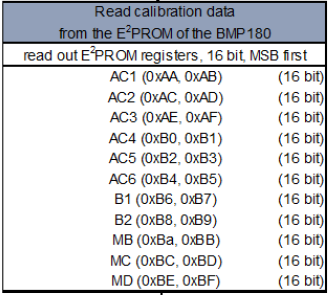
\includegraphics[width=200px]{calibracao_pressao_1.png}
  \caption{Registradores com dados de calibração}
  \label{calibracao_pressao_1}
\end{figure}

Depois de ler o valor medido pelo sensor e, de posse dos valores contidos nos registradores, basta seguir o algoritimo descrito na figura \ref{calibracao_pressao_2}.\par

\begin{figure}
  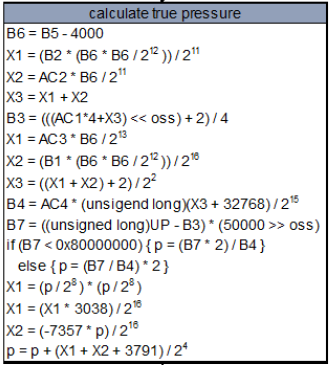
\includegraphics[width=200px]{calibracao_pressao_2.png}
  \caption{Calibração}
  \label{calibracao_pressao_2}
\end{figure}

A variável $UP$ é o valor lido pelo sensor, enquanto que as variáveis X1, X2, ... e B1, B2, ... são os valores dos registradores, conforme a figura \ref{calibracao_pressao_1}.\par

\subsection{Termômetro}\label{desenvolvimento_termometro}
O termômetro é um aparelho usado para medir a temperatura ou as variações de temperatura. É um instrumento composto por um elemento sensor que possua uma propriedade termométrica, isto é, uma propriedade que varia com a temperatura.\par
Dentro do formalismo da termodinâmica, que leva em conta apenas grandezas macroscopicamente mensuráveis, a temperatura é, de forma equivalente, definida como a derivada parcial da energia interna U em relação à entropia S para um sistema em equilíbrio termodinâminco, conforme a equação \ref{eq_temperatura}.\par

\begin{equation} \label{eq_temperatura}
T = \frac{\delta U(S)}{\delta S}
\end{equation}

No caso do nosso projeto, o sensor que utilizamos usa, de acordo com o datasheet \cite{ds18b22ds}, um protocolo de comunicação serial, enviando uma série de caracteres para controle de erro juntamente com a temperatura medida. Uma saída típica pode ser vista na figura \ref{saida_sensor_temperatura}.\par

\begin{figure}
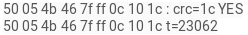
\includegraphics[width=200px]{sensor_temperatura.png}
\caption{Saída do sensor DS18B22}
\label{saida_sensor_temperatura}
\end{figure}

A temperatura fornecida pelo sensor pode ser utilizada apenas convertendo o valor fornecido para inteiro e, em seguida, dividindo por 1.000 e convertendo para ponto flutuante.\par

\subsection{Anemômetro}\label{desenvolvimento_anemometro}
Anemômetro é um instrumento utilizado para medir a velocidade de um fluido, como por exemplo ar ou água. Também pode ser utilizado em modelos físicos em laboratórios de hidráulica, de aerodinâmica ou, ainda, em qualquer outro fluido como os gases existentes em estrelas e planetas.\par
Neste trabalho não utilizamos nenhum sensor pronto para isso. Optamos por confeccionar o nosso próprio anemômetro utilizando uma chave óptica e uma haste com 3 pás.\par
Para medir a velocidade do vento, programamos que assim que a chave fosse acionada, uma interrupção seria disparada pelo microcontrolador, acionando uma rotina em nosso software. Essa rotina iniciaria um temporizador até a próxima interrupção, sinalizando uma volta completa. Esse processo é repetido pro 10 vezes, para termos um tempo médio. Então aplicamos a equação \ref{eq_frequencia} para termos a frequência (em Hz) para, então, aplicarmos a equação \ref{eq_velocidade_linear} para termos a velocidade do vento.\par

\begin{equation}
F = \frac{1}{t}
\label{eq_frequencia}
\end{equation}

\begin{equation}
  \omega = 2 \cdot \pi \cdot f
  \label{eq_velocidade_angular}
\end{equation}

\begin{equation}\label{eq_velocidade_linear}
\begin{split}
v &= \omega \cdot r \\
 &= 2 \cdot \pi \cdot f \cdot r
\end{split}
\end{equation}

Onde $f$ é a frequência calculada via software e $r$ é o raio do nosso anemômetro. O diâmetro do anemômetro foi medido com um paquímetro, obtendo-se $0,0321 m$, ou aproximadamente $0,023 m$.\par

Para sabermos se estávamos tendo medidas mais ou menos precisas, utilizamos um tacômetro para medir quantas revoluções por minuto (\textit{rpm}) nosso amemôtro estava fazendo quando ligamos um ventilador perto dele. Para isso, tivemos, também, que utilizar a equação \ref{eq_f_para_rpm} para transformar nossa frequência média em RPM.\par

\begin{equation}
  RPM = 60 \cdot f
  \label{eq_f_para_rpm}
\end{equation}

Com isso, notamos que conseguimos uma medida, via software, $\pm 2 RPM$ contra o tacômetro. Considerando-se o objetivo do projeto e os equipamentos utilizados, achamos este um erro satisfatório e pudemos proceder à próxima etapa dos testes do nosso anemômetro.\par

Montamos o anemômetro e o microcontrolador em uma placa de acrílico e dirigimos em trechos retos a uma velocidade constante, constrastando a medida da velocidade do software tanto com as medidas do velocímetro do carro, como com as medidas de um GPS. Coincidentemente, observamos um erro máximo de $\pm 5 km/h$, com a média em $\pm 2 km/h$.\par

Novamente, como o objetivo deste trabalho era construir uma estação meteorológica com IoT, e não um anemômetro preciso, consideramos essas medidas extremamente satisfatórias.\par

\subsection{Higrômetro}\label{desenvolvimento_higrometro}
Um higrômetro é um instrumento que serve para medir a umidade presente nos gases, mais especificamente na atmosfera. É utilizado principalmente em estudos do clima, mas também em locais fechados onde a presença de umidade excessiva ou abaixo do normal poderia causar danos, por exemplo, em peças de museus, documentos de bibliotecas e elementos de laboratórios.\par

\begin{equation}
  UR\% = \frac{e}{e_s} \cdot 100
  \label{eq_higrometro}
\end{equation}

A equação \ref{eq_higrometro} fornece a umidade relativa ($UR\%$) do ar em termos da pressão parcial de vapor de água do ar (g/kg), dado por $e$, e a pressão de vapor nas condições de equilíbrio, também chamada pressão de \textit{vapor de saturação}, dado por $e_s$, também medido em g/kg.\par

O sensor utilizado, o DHT22, utiliza um protocolo serial, ativado em nível lógico baixo. O funcionamento detalhado do sensor está descrito no datasheet \cite{dht22ds}, mas a figura \ref{protocolo_dht22} exibe o mesmo protocolo disponibilizado no datasheet.\par

\begin{figure}
  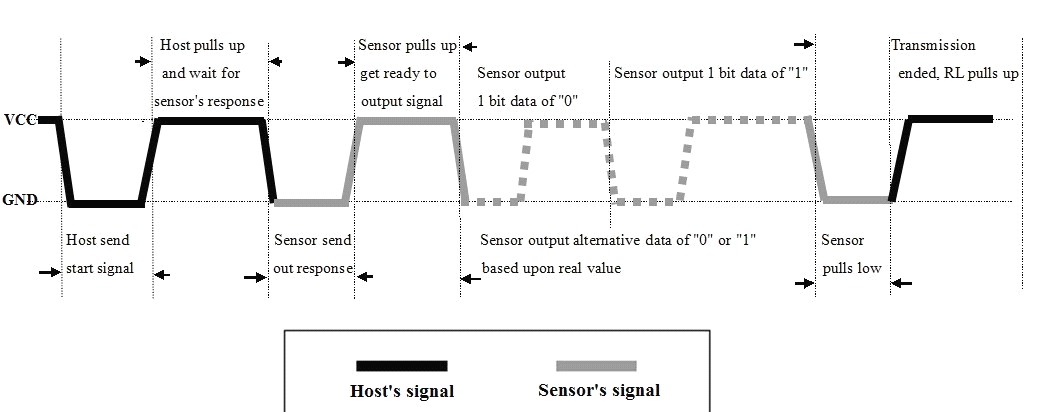
\includegraphics[width=200px]{sensor_umidade.png}
  \caption{Protocolo de transmissão do sensor DHT22}
  \label{protocolo_dht22}
\end{figure}

De acordo com o datasheet \cite{dht22ds}, "o estado de buffer sem dados é dado por um nível de tensão alto. Quando a comunicação entre o microcontrolador e o DHT22 inicia, o programa do microcontrolador irá passar o nível de tensão de alto para baixo por pelo menos 1 ms, para garantir que o DHT22 detecte o sinal do microcontrolador, então o microcontrolador irá esperar entre 20 a 40 $\mu s$ pela resposta do DHT22"\footnote{Data-bus' free status is high voltage level. When communication between MCU and DHT22 begin, program of MCU will transform data-bus' voltage level from high to low level and this process must beyond at least 1ms to ensure DHT22 could detect MCU's signal, then MCU will wait 20-40 $\mu s$ for DHT22's response.} (tradução nossa).

\subsection{Software}\label{sw}
\subsubsection{Protocolo}\label{sw_protocolo}
Um dos protocolos de troca de mensagens para IoT em uso recente é o MQTT(Message Queue Telemetry Transport). Criado pela IBM no final da década de 90, obviamente o protocolo carrega muito do cenário de uso original, mais voltado e adaptado para sistemas de supervisão e coleta de dados do tipo SCADA (Supervisory Control and Data Acquisition ou Sistemas de Supervisão e Aquisição de Dados). Mas, mesmo assim, o MQTT encontrou seu espaço nesse amplo mercado de IoT.\par
O padrão de troca de mensagens no MQTT é o publish / subscriber (publicador / subscritor). Neste padrão, quando um elemento da rede deseja receber uma determinada informação, ele a subscreve, fazendo uma requisição para um outro elemento da rede capaz de gerir as publicações e subscrições. Na rede MQTT este elemento é conhecido como broker, o intermediário no processo de comunicação. Elementos que desejam publicar informações o fazem também através do broker, enviando-lhe as informações que possuem. Esse padrão não é novo e existe em outros protocolos. Por exemplo, a troca de informação de controle (links) em redes Foundation Fieldbus segue o paradigma publish / subscriber.\par
A identificação das mensagens no MQTT se dá através de tópicos (topics). O tópico lembra o conceito de URI, com níveis separados por barras ("/"). Elementos da rede podem enviar diversos tópicos para o broker e subscritores podem escolher os tópicos que desejam subscrever.\par
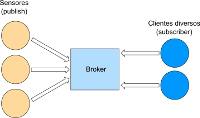
\includegraphics{mqtt_small.png}

Em nosso projeto, definimos que cada sensor publicaria sua medida em um sub-tópico específico: $temperatura$, $pressao$, $umidade$ e $vento$. O tópico principal foi nomeado como $estacao$. Dessa forma, é possível realizar a leitura em qualquer cliente MQTT sem definir um protocolo específico e sem a necessidade de ter um cliente específico para a estação.\par

\subsection{Conectividade}\label{sw_conectividade}
Utilizamos o módulo interno de conectividade wireless da Raspberry. Com isso, utilizando um celular como roteador, pudemos conectar à internet, e enviar as medidas via MQTT, sempre que o celular estivesse disponível. A utilização de wireless ao invés de cabos foi, como esperado, completamente transparente ao software.\par

\subsection{Desenvolvimento}\label{sw_desenvolvimento}
Optamos por utilizar a linguagem C, conforme a seção \ref{desenvolvimento}, por ser uma linguagem leve e de rápido desenvolvimento, bem como esparsa documentação.\par
Cada sensor teve seus algoritimos desenvolvidos em um arquivo à parte, sendo todos eles interligados, ao final, por um arquivo $main.c$, responsável pela inicialização de periféricos comuns, parâmetros de configuração globais e inicialização das threads de cada sensor.\par
Cada módulo de sensor, portanto, era executado em uma thread separada, garantindo isolamento de processos e recursos, bem como garantindo que um erro em um sensor não afetaria o funcionamento dos demais.\par
A Raspberry foi, então, configurada para iniciar o software tão logo o boot do sistema embarcado fosse concluído, garantindo, assim, que o sistema não dependesse de um teclado e monitor para funcionar. Para garantir o funcionamento do software, utilizamos um \textit{LED} e um padrão luminoso, definido por nós mesmos, para identificar em qual etapa de inicialização o software se encontra. Ao final da inicialização, o \textit{LED} permanece acesso enquanto o sistema estiver operante.\par

\section{Conclusão}\label{conclusao}
A confecção modular do sistema facilitou os ensaios e as conclusões de cada etapa. Assim que cada módulo estava funcionando, conectar ao todo era um passo muito trivial, o que permitiu concluir o projeto antes do prazo de entrega.\par
O sensor DHT22, mostrou-se instável em alguns momentos, chegando até a parar de funcionar. Foi quando uma pesquisa ao datasheet trouxe a informação que este sensor pode ficar inoperante por até 5 horas, se exposto a grandes variações de temperatura, exatamente o que aconteceu em um dos testes, quando expusemos todo o sistema à um ventilador para calibração do anemômetro.\par
Apesar de não estar previsto no projeto inicial, foi adicionado um barômetro, complementando a estação IoT com mais essa aquisição de pressão, que é de extrema importância em um sistema meteorológico.\par
A montagem final pode ser conferida na figura \ref{montagem_final}.

\begin{figure}
  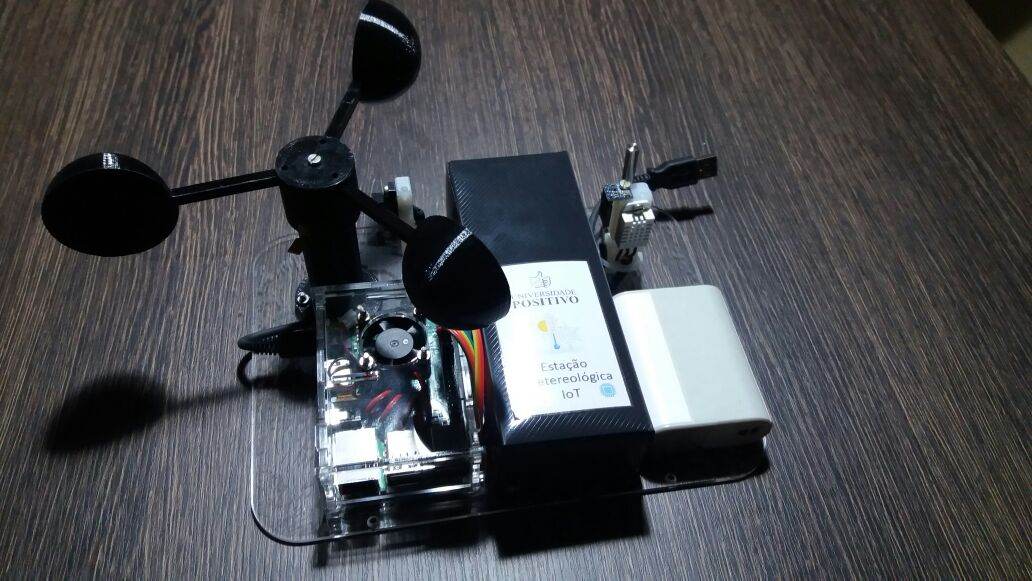
\includegraphics[width=200px]{estacao_final.jpeg}
  \caption{Montagem final da estação meteorológica}
  \label{montagem_final}
\end{figure}

\begin{thebibliography}{9}
\bibitem{dht22ds}
Aosong Electronics.
Datasheet: Digital-output relative humidity \& temperature sensor/module DHT22.
Disponível em: \url{https://www.sparkfun.com/datasheets/Sensors/Temperature/DHT22.pdf}.
Acesso em 16/11/2017.
\bibitem{bmp180ds}
Bosch Sensortec.
Datasheet:BMP180 Digital pressure sensor.
Disponível em: \url{https://cdn-shop.adafruit.com/datasheets/BST-BMP180-DS000-09.pdf}.
Acesso em 16/11/2017.
\bibitem{ds18b22ds}
Maxim Integrated.
Datasheet: DS18B20 Programmable Resolution 1-Wire Digital Thermometer.
Disponível em: \url{http://datasheets.maximintegrated.com/en/ds/DS18B20.pdf}.
Acesso em 16/11/2017.
\bibitem{wikiestacao}
Wikipedia.
Estação Meteorológica.
Disponível em: \url{https://pt.wikipedia.org/wiki/Esta%C3%A7%C3%A3o_meteorol%C3%B3gica}.
Acesso em 16/11/2017.
\end{thebibliography}
\end{document}
